\section{Application to a Domain Decomposition Method}

\indent The constant polynomial approximation of the Transparent Boundary Conditions, expressed by \ref{eq:TBC3}, will be applied to the implementation of a Domain Decomposition Method (DDM). Firstly, we will briefly describe the DDM that we will consider here, and after we will describe and test the incorporation of the proposed TBCs.

\subsection{The Schwarz Methods}

\indent The following description is based on \cite{Japhet2003}. Domain Decomposition Methods allow to decompose a domain $\Omega$ in multiple subdomains $\Omega_i$ (that can possibly overlap) and solve the problem in each one of them. Therefore, one must find functions that satisfies the PDE in each subdomain and that match on the interfaces. 

\indent The first DDM developed was the Schwarz method, which consists on an iterative method : in the case of a evolution problem, the solution  $u_i^{n,\infty}$, in each time step $t_n$ and each subdomain $\Omega_i$, is computed as the convergence of the solution obtained in each iteration, $u_i^{n,k}, \ \ k\geq 0$. There are two types of Schwarz methods, depending on the way that the boundary conditions on the interfaces are constructed for computing $u_i^{n,k}$

\indent We will consider her the additive Schwarz method (ASM), in which the boundary conditions are always constructed using the solution $u_j^{n,k-1}, \ \ j \neq i$ of the previous iteration in the other partitions of the domain. Therefore, in each interface between the domains $\Omega_i$ and $\Omega_j$, the boundary condition for the problem in $\Omega_i$ is

$$\mathcal{B}(u_i^{n,k+1}) = \mathcal{B}(u_j^{n,k})$$

\noindent where $\mathcal{B}$ denotes the operator of the TBC.

%\indent In the order hand, the multiplicative Schwarz method (MSM) uses always the most recent information for computing the interface boundary conditions. Therefore, if we consider a DDM with two subomains, $\Omega_1$ and $\Omega_2$,  they TBCs would be written (for example) as 

%$$\mathcal{B}(u_1^{n,k+1}) = \mathcal{B}(u_2^{n,k}) \\ \mathcal{B}(u_2^{n,k+1}) = \mathcal{B}(u_1^{n,k+1})$$

%\noindent for solving the problem in $\Omega_1$ and $\Omega_2$, respectively.

%\indent We will consider here only the ASM.In the following description, without lost of generality, we will consider a domain decomposed in two non-overlapping subdomains.

\indent Without loss of generality, in the following we will consider a domain decomposed in two non-overlapping subdomains.

\indent Evidently, the biggest challenge of the Schwarz methods is to define appropriate operators such that :

\begin{itemize}
\item The method shows a fast convergence
\item The solution $u_i$ in each subdomain $\Omega_i$ converges to $u|_{\Omega_1}$, i.e, the solution $u$ of the monodomain $\Omega$ restricted to $\Omega_1$
\end{itemize} 

\indent In fact, accordingly to \cite{Japhet2013}, the optimal additive Schwarz method is the one which uses the TBCs \ref{REFTBCMAY} as interface boundary conditions: with them, the method converges in two iterations, and no ASM can converge in less than two iterations.

\indent Nevertheless, as discussed previously in this report, the numerical implementation of the exact TBCs \ref{REFTBCMAY} are generally impractical, because they are non local in time. Therefore, one should use approximate TBCs, what will be done here in the sequence using the approximations proposed n the previous section.

\subsection{ASM with the approximate TBCs for the dispersive equation}

\indent The resolution of the dispersive equation with the Additive Schwarz method, using the constant polynomial approximation for the TBCs, is written as

\begin{equation}
    \label{eq:problemDDM1}
    \begin{cases}
        (u_1^{n,k+1})_t + (u_1^{n,k+1})_{xxx} = 0 , \ \ x \in \Omega_1, \ \ t \leq 0\\
        u_1^{n,0} = u_1^{n-1,\infty} , \ \ x \in \Omega_1 \\
        \Upsilon_1^{c_L^*}(u_1^{n+1,k+1},-L) = 0, \\ 
        \Theta_2^{c_R^*}(u_1^{n+1,k+1},0) = \Theta_2^{c_R^*}(u_2^{n,k},0) , \\
        \Theta_3^{c_R^*}(u_1^{n+1,k+1},0) = \Theta_3^{c_R^*}(u_2^{n,k},0)
     \end{cases}
\end{equation}

\begin{equation}
    \label{eq:problemDDM2}
    \begin{cases}
        (u_2^{n,k+1})_t + (u_2^{n,k+1})_{xxx} = 0 , \ \ x \in \Omega_2, \ \ t \leq 0\\
        u_2^{n,0} = u_2^{n-1,\infty} , \ \ x \in \Omega_2 \\
        \Theta_1^{c_L^*}(u_2^{n+1,k+1},0) = \Theta_1^{c_L^*}(u_1^{n,k},0) \\
        \Upsilon_2^{c_R^*}(u_2^{n+1,k+1},L) = 0 \\
        \Upsilon_3^{c_R^*}(u_2^{n+1,k+1},L) = 0
     \end{cases}
\end{equation}

\indent where $ \Upsilon_i, \ \ i=1,2,3$, are the boundary conditions on the external boundaries (i.e, in the intersection of the monodomain boundaries and the subdomain boundaries). These external BCs are independent of the interface BCs. Here, we will consider $\Upsilon_1 = \Theta_1^{1.0}$, $\Upsilon_2 = \Theta_2^{0.0}$ and $\Upsilon_3 = \Theta_3^{0.0}$, which gives

\begin{gather}
	\Upsilon_1(u,x) = u - u_x + u_{xx} \\
	\Upsilon_2(u,x) = 0 \\
	\Upsilon_3(u,x) = 0 \\
\end{gather}

\indent This choice was made based on the easy implementation and the good results provided by the coefficients $c_L = 1.0$ and $c_R = 0.0$ in approximating the analytical solution in $\Omega$ (as shown in the table \ref{tab:firstTestsP0}). Nevertheless,it does not have much importance in the study that we will done in the following paragraphs. In fact, our purpose is to study exclusively the behavior of the DDM implemented here; therefore, all the results must be compared to a referential solution $u_{ref}$, that can be simply the numerical solution of the monodomain problem. The only restriction for an appropriate study is that the external BCs for computing $u_{ref}$ must be same as $\Upsilon_i, \ \ i=1,2,3$.

\subsection{Error in the converged solution}

\indent When using approximate TBCs in the ASM, one should guarantee that the converged solutions $u_1,u_2$ satisfies the same equation as the solution $u_{ref}$ of the monodomain problem. In the following paragraphs, we show that this property is not verified by the method \eqref{eq:problemDDM1} - \eqref{eq:problemDDM2} proposed here. Based on that, we will be able to propose corrections for it.


\subsubsection{Study of the error in the DDM method for the dispersion equation}

\indent Now we will apply a similar idea to study the error of the Domain Decomposition Method that we proposed for the dispersive equation. As mentioned above, we will focus exclusively on the error produced by DDM, independently of the other possible components of the error compared to the exact solution for the example (external boundary conditions, error accumulation over the time steps). Therefore, all the following study will be made considering the execution of the method over only one time step, allowing us to use a clearer notation for the solution : $u_j^i$, where $i$ indicates the subdomain $\Omega_i$ and $j$ indicates the spatial discrete position. In the cases where the iterative process is take in account, we will add the superscript $k$ to indicate the iteration.

\indent For the interior points of each one of the domains, we will consider a second order spatial discretization of the equation (\ref{eq:linearizedKdV}).

\begin{equation}
    \label{eq:FDdiscretization}
    \frac{u_j^i - \alpha_j^i}{\Delta t} + \frac{-\frac{1}{2}u_{j-2}^i + u_{j-1}^i - u_{j+1}^i + \frac{1}{2}u_{j+2}^i }{\Delta x ^3} = 0
\end{equation}

\indent for $j=2,...,N-2$ in the case $i=1$; for $j=N+2,...,2N-2$ in the case $i=2$; and for $j=2,...,2N-2$ in the case $i=ref$. In the above expression, $\alpha_j^i$ is a given data (for example, the converged solution in the previous time step).

\indent For the points near the boundaries, we use second order uncentered discretizations or the appropriate TBCs. We will focus here on the interface point $x_N$. Thus, in the resolution of the problem in $\Omega_1$, two interface boundary conditions are imposed (corresponding to $\Theta_2$ and $\Theta_3$), so the solutions $u_{N-1}^1$ and $u_N^1$ are computed using the equations

\begin{equation}
	\begin{aligned}
    \label{eq:TBCsIterOmega1A}
    && 				&\Theta_2^{c_R}(u_N^1) = \Theta_2^{c_R}(u_N^2) \implies \\ 
    && \implies & u_N^1 - c_R^2 \frac{u_N^1 - 2u_{N-1}^1 + u_{N-2}^1}{\Delta x^2} = u_N^2 - c_R^2 \frac{u_N^2 - 2u_{N+1}^2 + u_{N+2}^2}{\Delta x^2} 
    \end{aligned}
\end{equation}

\begin{equation}
	\begin{aligned}
    \label{eq:TBCsIterOmega1B}
    && 			   & \Theta_3^{c_R}(u_N^1) = \Theta_3^{c_R}(u_N^2) \implies \\
    && \implies & \frac{u_N^1 - u_{N-1}^1}{\Delta x} + c_R \frac{u_N^1 - 2u_{N-1}^1 + u_{N-2}^1}{\Delta x^2} = \frac{u_{N+1}^2 - u_{N}^2}{\Delta x} + c_R \frac{u_N^2 - 2u_{N+1}^2 + u_{N+2}^2}{\Delta x^2}
    \end{aligned}
\end{equation}

\indent In the resolution of the problem in $\Omega_2$, only one interface boundary condition is used (corresponding to $\Theta_1$) :

\begin{equation}
	\begin{aligned}
    \label{eq:TBCsIterOmega2}
    && 				&\Theta_3^{c_L}(u_N^2) = \Theta_3^{c_L}(u_N^1) \implies \\ 
    && \implies & u_N^2 - c_L \frac{u_{N+1}^2 - u_{N}^2}{\Delta x} + c_L^2 \frac{u_N^2 - 2u_{N+1}^2 + u_{N+2}^2}{\Delta x^2}  =\\
    && 				& u_N^1 - c_L \frac{u_{N}^1 - u_{N-1}^1}{\Delta x} + c_L^2 \frac{u_N^1 - 2u_{N-1}^1 + u_{N-2}^1}{\Delta x^2}
    \end{aligned}
\end{equation}

\indent In the convergence, \eqref{eq:TBCsIterOmega1A} to\eqref{eq:TBCsIterOmega2} gives respectively

\begin{equation}
    \label{eq:TBCsCVOmega1A}
\begin{aligned}
    && 			    &u_N^* - c_R^2 \frac{u_N^* - 2u_{N-1}^* + u_{N-2}^*}{\Delta x^2} = u_N^* - c_R^2 \frac{u_N^* - 2u_{N+1}^* + u_{N+2}^*}{\Delta x^2} \implies  \\
    && \implies & 2c_R^2 \frac{-\frac{1}{2}u_{N-2}^* + u_{N-1}^* - u_{N+1}^* + \frac{1}{2}u_{N+2}^* }{\Delta x^2} = 0
    \end{aligned}
    \end{equation}
    
\begin{equation}
    \label{eq:TBCsCVOmega1B}
\begin{aligned}
    &&             &\frac{u_N^* - u_{N-1}^*}{\Delta x} + c_R \frac{u_N^* - 2u_{N-1}^* + u_{N-2}^*}{\Delta x^2} = \\
    && 			   &\frac{u_{N+1}^* - u_{N}^*}{\Delta x} + c_R \frac{u_N^* - 2u_{N+1}^* + u_{N+2}^*}{\Delta x^2} \implies \\
    && \implies & -\frac{u_{N-1}^* - 2 u_{N}^* + u_{N+1}^*}{\Delta x} - 2c_R\frac{-\frac{1}{2}u_{N-2}^* + u_{N-1}^* - u_{N+1}^* + \frac{1}{2}u_{N+2}^* }{\Delta x^2} = 0 
\end{aligned}
\end{equation}

\begin{equation}
    \label{eq:TBCsCVOmega2}
\begin{aligned}
   && 					&	 u_N^* -  c_L\frac{u_{N+1}^* - u_{N}^*}{\Delta x} + c_L^2 \frac{u_{N}^* - 2u_{N+1}^* + u_{N+2}^*}{\Delta x^2} = \\ 
   && 					& u_N^* -  c_L\frac{u_{N}^* - u_{N-1}^*}{\Delta x} + c_L^2 \frac{u_{N}^* - 2u_{N-1}^* + u_{N-2}^*}{\Delta x^2} \implies \\
	&&  \implies	    & -c_L\frac{u_{N-1}^* - 2 u_{N}^* + u_{N+1}^*}{\Delta x} + 2c_L^2\frac{-\frac{1}{2}u_{N-2}^* + u_{N-1}^* - u_{N+1}^* + \frac{1}{2}u_{N+2}^* }{\Delta x^2} = 0 
\end{aligned}
\end{equation}

\indent Therefore, we can see that, the converged solution of the DDM method satisfies the same equation as the reference solution in all the points $x_j \in \Omega_1$, except in $x_{N-1}$ and $x_N$ (for the problem solved in $\Omega_1$) and in $x_N$ (for the problem solved in $\Omega_2$) . For example, it's easy to verify that \eqref{eq:TBCsCVOmega1A} differ from \eqref{eq:FDdiscretization} by a $O(\Delta x)$ term :

\begin{equation}
    \label{eq:diffEquations}
    \begin{aligned}
    2\Delta x c_R^2\left( \frac{u_N^* - \alpha_N^*}{\Delta t} + \frac{-\frac{1}{2}u_{N-2}^* + u_{N-1}^* - u_{N+1}^* + \frac{1}{2}u_{N+2}^* }{\Delta x ^3} \right) - \\
    \left( 2c_R^2 \frac{-\frac{1}{2}u_{N-2}^* + u_{N-1}^* - u_{N+1}^* + \frac{1}{2}u_{N+2}^* }{\Delta x^2} \right) =  2\Delta x c_R^2 \frac{u_N^* - \alpha_N^*}{\Delta t}
    \end{aligned}
\end{equation}

\paragraph{Numerical verification of the error}

\indent The problem \eqref{eq:problemDDM1} - \eqref{eq:problemDDM2} was solved until the convergence with 5 different uniform spatial discretizations, over one time step (in the interval $[0,\Delta t]$). In each case, the adopted referential solution $u^{ref}$ was the monodomain problem, solved with the same mesh size. Two errors were computed : 

\begin{equation}
	e^{N,\Omega_1\bigcap \Omega_2} = |u^{ref}_N - u^{1}_N|
\end{equation}

\begin{equation}
	e^{N,\Omega} = ||u^{ref}_N - u^{1,2}_N||_2 = \sqrt{dx}\sqrt{\sum_{j=0}^N{(u^{ref}_j - u^{1}_j)^2 } + \sum_{j=N}^{2N}{(u^{ref}_j - u^{2}_j)^2 } }
\end{equation}

\noindent corresponding respectively to the error on the interface and the error on the whole domain. In the notation $e^{N,\bullet}$, $N$ refers to the number of space steps in $\Omega$.

\indent We are interested in the behavior of these error as the mesh size changes. As shown in the table \ref{fig:orderVerification}, we verify that the DDM proposed here produces a first order error :

\begin{center}
	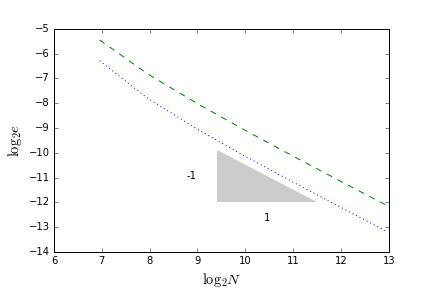
\includegraphics[scale=.5]{figures/convergenceVerification.png}
	\captionof{figure}{Numerical verification of the order of convergence of the error due to the Domain Decomposition Method \label{fig:orderVerification}}
\end{center}

\subsubsection{Corrections for the approximate TBCs}

\indent Then, we will formulate modified TBCs for the ASM method in order to cancel these errors :

\begin{equation}
    \begin{cases}
        \Theta_1^{c_L^*}(u_2^{n+1,k+1},0) + \theta_1 = \Theta_1^{c_L^*}(u_1^{n,k},0) + \theta_1' \\
        \Theta_2^{c_R^*}(u_1^{n+1,k+1},0) + \theta_2 = \Theta_2^{c_R^*}(u_2^{n,k},0) + \theta_2' \\
        \Theta_3^{c_R^*}(u_1^{n+1,k+1},0) + \theta_3 = \Theta_3^{c_R^*}(u_2^{n,k},0) + \theta_3'
    \end{cases}
\end{equation}

\noindent with $\theta_i, \theta_i'$ derived below, after a numerical verification of the error produced by the DDM.


\paragraph{Determination of $\theta_1, \theta_1'$}

\indent Our objective is to write (\ref{eq:FDdiscretization}) in the point $x_{N}$ :

\begin{equation}
    \label{eq:FDdiscretizationN}
    \frac{u_{N}^* - \alpha_{N}^*}{\Delta t} + \frac{-\frac{1}{2}u_{N-2}^* + u_{N-1}^* - u_{N+1}^* + \frac{1}{2}u_{N+2}^* }{\Delta x ^3} = 0
\end{equation}

\indent Defining 

\begin{gather}
    \theta_1 = c_L \frac{u_{N+1}^2 - u_{N}^2}{\Delta x} + c_L^2\frac{\Delta x}{\Delta t} \left( u_{N}^2 - \alpha_{N}^2 \right)\\
    \theta_1' = c_L \frac{u_{N}^1 - u_{N-1}^1}{\Delta x} - c_L^2\frac{\Delta x}{\Delta t} \left( u_{N}^1 - \alpha_{N}^1 \right)
\end{gather}

\indent we have, in the convergence, that

\begin{equation}
\label{eq:modifiedTBC1}
\begin{aligned}
&& &    \Theta_1^{c_L}(u_N^*) + \theta_1 = \Theta_1^{c_L}(u_N^*) + \theta_1'\implies \\
&& \implies &    u_N^* - c_L \frac{u_{N+1}^* - u_N^*}{\Delta x} + c_L^2\frac{u_N^* - 2u_{N+1}^* + u_{N+2}^*}{\Delta x^2} + c_L \frac{u_{N+1}^* - u_{N}^*}{\Delta x} + c_L^2\frac{\Delta x}{\Delta t} \left( u_{N}^* - \alpha_{N}^* \right) = \\
&& & u_N^* - c_L \frac{u_{N}^* - u_{N-1}^*}{\Delta x} + c_L^2\frac{u_N^* - 2u_{N-1}^* + u_{N-2}^*}{\Delta x^2} + c_L \frac{u_{N}^* - u_{N-1}^*}{\Delta x} - c_L^2\frac{\Delta x}{\Delta t} \left( u_{N}^* - \alpha_{N}^* \right) \implies \\
 && \implies &    2c_L^2 \frac{-\frac{1}{2}u_{N-2}^* + u_{N-1}^* - u_{N+1}^* + \frac{1}{2}u_{N+2}^* }{\Delta x ^2}  +             2c_L^2\frac{\Delta x}{\Delta t} \left( u_{N}^* - \alpha_{N}^* \right) = 0 \implies \\
&& \implies &    \frac{u_{N}^* - \alpha_{N}^*}{\Delta t} + \frac{-\frac{1}{2}u_{N-2}^* + u_{N-1}^* - u_{N+1}^* + \frac{1}{2}u_{N+2}^* }{\Delta x ^3} = 0
\end{aligned}
\end{equation}

\noindent which corresponds to the discretization \eqref{eq:FDdiscretization} satisfied in $x_N$. 

\paragraph{Determination of $\theta_2, \theta_2'$}

\indent Based on \eqref{eq:diffEquations}, we define

\begin{equation}
\begin{gathered}
    \theta_2 = \frac{\Delta x}{\Delta t} c_R^2 (u_N^1 - \alpha_N^1) \\
    \theta_2' = -\frac{\Delta x}{\Delta t} c_R^2 (u_N^2 - \alpha_N^2)
\end{gathered}
\end{equation}

\indent Indeed, we then have, in the convergence

\begin{equation}
\label{eq:modifiedTBC2}
\begin{aligned}
&& &\Theta_2^{c_R}(u_N^*) + \theta_2 = \Theta_2^{c_R}(u_N^*) + \theta_2'\implies \\
&& \implies & u_N^* - c_R^2 \frac{u_N^* - 2u_{N-1}^* + u_{N-2}^*}{\Delta x^2} + \frac{\Delta x}{\Delta t} c_R^2 (u_N^* - \alpha_N^*)  = \\ && & u_N^* - c_R^2 \frac{u_N^* - 2u_{N+1}^* + u_{N+2}^*}{\Delta x^2} -\frac{\Delta x}{\Delta t} c_R^2 (u_N^* - \alpha_N^*) \implies \\
&& \implies & 2\frac{\Delta x}{\Delta t} c_R^2 (u_N^* - \alpha_N^*) + 2c_R^2 \frac{-\frac{1}{2}u_{N-2}^* + u_{N-1}^* - u_{N+1}^* + \frac{1}{2}u_{N+2}^* }{\Delta x^2} = 0  \implies \\
&& \implies &\frac{u_N^* - \alpha_N^*}{\Delta t} + \frac{-\frac{1}{2}u_{N-2}^* + u_{N-1}^* - u_{N+1}^* + \frac{1}{2}u_{N+2}^* }{\Delta x^3} = 0
\end{aligned}
\end{equation}

\noindent which corresponds to the discretization \eqref{eq:FDdiscretization} satisfied in $x_N$.


\paragraph{Determination of $\theta_3, \theta_3'$}

\indent Using \eqref{eq:modifiedTBC2} in \eqref{eq:TBCsIterOmega1B}, we get

\begin{equation}
-\frac{u_{N-1}^* - 2 u_{N}^* + u_{N+1}^*}{\Delta x} + 2c_R\Delta x\frac{u_N^* - \alpha_N^*}{\Delta t} = 0 
\end{equation}

\indent Now, our objective is to write \eqref{eq:FDdiscretization} in the point $x_{N-1}$ :

\begin{equation}
    \label{eq:FDdiscretizationNm1}
    \frac{u_{N-1}^* - \alpha_{N-1}^*}{\Delta t} + \frac{-\frac{1}{2}u_{N-3}^* + u_{N-2}^* - u_{N}^* + \frac{1}{2}u_{N+1}^* }{\Delta x ^3} = 0
\end{equation}

\noindent what can be achieved by defining

\begin{equation}
\begin{gathered}
    \theta_3 = 2\frac{\Delta x}{\Delta t} \left[-\Delta x(u_{N-1}^1 - \alpha_{N-1}^1) - c_R (u_N^1 - \alpha_N^1) \right] + \frac{u_{N-3}^1 - 2u_{N-2}^1 + u_{N-1}^1}{\Delta x} \\
    \theta_3' = 0
\end{gathered}
\end{equation}

\indent In fact, in the convergence,

\begin{align*}
\label{eq:modifiedTBC3}
&&  &\Theta_3^{c_R}(u_N^*) + \theta_3 = \Theta_3^{c_R}(u_N^*) + \theta_3'     \implies \\
&& \implies & \frac{u_N^* - u_{N-1}^*}{\Delta x} + c_R \frac{u_N^* - 2u_{N-1}^* + u_{N-2}^*}{\Delta x^2} + 2\frac{\Delta x}{\Delta t}  \left[-\Delta x(u_{N-1}^* - \alpha_{N-1}^*) - c_R (u_N^* - \alpha_N^*) \right] + \\
&&   & 			\frac{u_{N-3}^* - 2u_{N-2}^* + u_{N-1}^*}{\Delta x}  =  \frac{u_{N+1}^* - u_{N}^*}{\Delta x} + c_R \frac{u_N^* - 2u_{N+1}^* + u_{N+2}^*}{\Delta x^2} \implies \\
&&  \implies &  -\frac{u_{N-1}^* - 2 u_{N}^* + u_{N+1}^*}{\Delta x} + 2c_R\Delta_x\frac{u_N^* - \alpha_N^*}{\Delta t} + \\
&&   & 2\frac{\Delta x}{\Delta t} \left[-\Delta x(u_{N-1}^* - \alpha_{N-1}^*) - c_R(u_N^* - \alpha_N^*) \right] + \frac{u_{N-3}^* - 2u_{N-2}^* + u_{N-1}^*}{\Delta x} = 0 \implies \\
&& \implies  & -2\frac{-\frac{1}{2}u_{N-3}^* + u_{N-2}^* - u_{N}^* + \frac{1}{2}u_{N+1}^* }{\Delta x} - 2\frac{\Delta x^2}{\Delta t}(u_{N-1}^* - 					\alpha_{N-1}^*) = 0 \implies \\
&& \implies &  \frac{u_{N-1}^* - \alpha_{N-1}^*}{\Delta t} + \frac{-\frac{1}{2}u_{N-3}^* + u_{N-2}^* - u_{N}^* + \frac{1}{2}u_{N+1}^* }{\Delta x ^3} = 0
\end{align*}

\paragraph{Modification of the reference solution}

\indent The modifications proposed above for the CBCs effectively allows the points $x_{N-1},x_N \in \Omega_1$ and $x_N \in \Omega_2$ to satisfy the same discrete equation as in the monodomain problem. Nevertheless, the solution of the DDM does not converge exactly to $u^{ref}$, for a reason that does not depend on the expression of the CBCs, but on the fact that for each domain we write two CBCs in the left boundry and only one on the right. We are using a second order centered discretization for the third spatial derivative (which uses a stencil of two points in each side of the central point), which implies that we must write an uncentered discretization for the point $x_{N+1}$ when solving the problem in $\omega_2$. Therefore, this point does not satisfy the same discrete equation. In order to avoid this problem and allow us to verify that our method is able to correct the error of the DDM, we modify the discretization for the point $u_{N+1}$ in the monodmoain problem, using the same second-order uncentered expression 

\begin{equation}
    \label{eq:uncenteredFDdiscretizationN}
    \frac{u_{N+1}^2 - \alpha_{N+1}^2}{\Delta t} + \frac{-\frac{5}{2}u_{N+1}^2 + 9u_{N+2}^2 - 12 u_{N+3}^2 + 7\frac{1}{2}u_{N+4}^2 -\frac{3}{2}u_{N+1}^2}{\Delta x ^3} = 0
\end{equation}

\subsection{Optimization of the CBCs (speed of convergence)}

\indent Our objective now is to optimize the CBCs in the sense of minimizing the number of iterations of the ASM until the convergence. Therefore, similarly to the optimization of the TBCs made in the section \ref{sec:TBC}, we will made a very large set of tests in order to find the coefficients $c_L$ and $c_R$ (i.e., the constant polynomial approximation for the TBC) that provides the fastest convergence. In a first moment, we will make this study with fixed time step and space step, in order to analyze exclusively the influence of the coefficient, and after we will introduce these two parameters into the study.

\indent As we are interested in the speed with which the solution of the DDM method converges to the reference solution, the criteria of convergence used is

\begin{equation}
\label{eq:criteriaConvergence}
	e^k = ||\tilde{u}^{k,DDM} - \tilde{u}^{k,ref}||_2 = \sqrt{\Delta x \left[ \sum_{j=0}^{N}{\left(u^{k,1}_j - u^{k,ref}_j \right)^2} + \sum_{j=N}^{2N}{\left(u^{k,2}_j - u^{k,ref}_j \right)^2} \right]} 
\end{equation}
